%************************************************
\chapter{Hydrogen Bonding in Alcohol}
%************************************************
\begin{flushright}
September 27, 2012
\end{flushright}
\section{Objective}
To study the hydrogen bonds in alcohols using infrared spectroscopy.

\section{Theory}
	Alcohols in liquid form, interact via hydrogen bonds. This interaction results in a broad peak in the spectrum of alcohols, near the $O-H$ stretching region, viz. 3500 $cm^{-1}$.
	\par
	To verify this theory, we dilute the alcohol progressively in $CCl_{4}$ and expect the peak to get narrower as fewer interactions take place, with lower concentration. One may argue that the intensity of the peak will also drop. However, this method increases `contrast' at the expense of `brightness', viz. the peak relative to the rest of the spectra will continue to be observable and its spread is expected to decrease.
	\par
	We used Methanol in our experiment. Hydrogen bonds form as shown in \autoref{4B_Bonds}
	\par
	\subsubsection{A Little Deeper}
		The monomeric alcohol is responsible for producing a sharp peak. The broadening is attributed to the associated alcohol. However, that's not it. Now let's consider a broad peak. Here, the maxima will correspond to the associated molecules, with $O-H$ vibrating with an energy corresponding to that particular wavenumber, where the peak is observed. We can safely conclude that due to association, the molecules will vibrate with lower energy and can therefore expect the peak to be red shifted, with respect to the sharp peak of monomeric alcohol.
		\par
		Also, its natural to conclude that the broadness and extent of shift signifies the extend of hydrogen bonding and/or association of alcohol under investigation.

	\begin{figure}[bth]
		\begin{center}
			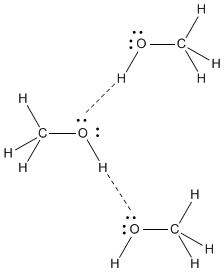
\includegraphics[width=0.3\linewidth]{gfx/4B}
		\end{center}
	\caption[Hydrogen Bonds in Methanol]{\label{4B_Bonds}}
	\end{figure}


\section{Procedure}
	We took Methanol (other groups took Ethanol and Propanol because the analysis takes longer, so all groups couldn't afford to 2) and $CCl_{4}$ and three 10 $mL$ volumetric flasks. \footnote{Reformulated from Prof. KS Viswanathan's Notes}
	\begin{enumerate}
		\item In the first, pipetted 0.5 $mL$ of alcohol and made up the volume using $CCl_{4}$. Labelled this as Solution A.
		\item In the second, took 5 $mL$ of solution A and made up the volume again using $CCl_{4}$. Labelled this as solution B.
		\item In the third, took 5 $mL$ of solution B and made up the volume as before.
	\end{enumerate}
	Recorded the IR Spectra of the solutions prepared above, and of neat alcohol {\marginpar{\Lisa Neat here means undiluted.}}. Then compared the spectra for varying concentrations and compared the characteristics of the peak corresponding to hydrogen bonding.
% Propenol 3625
% Ethenol  
\section{Observations/Discussion}
	The graphs and observations have been attached herewith, however they do not seem to be consistent with the thoery. Since K. S. Visvanathan sir was not in the campus until the date of submission, I couldn't understand how to interpret the data.

\section{Acknowledgements}
I thank our Lab Assistant, Mr. Mangat Kashyap, who helped us with the performance of the UV-Vis Spectroscopy. I also acknowledge the contribution of my team members, Ms. Athira and Mr. Arpit, for performance of the experiment.

\section{References}
	\begin{enumerate}
		\item K. S. Visvanathan's Notes
	\end{enumerate}